% !TEX root =  ../main_manuscript.tex 
\subsection{Statistical Model}
To create personalized biopsy schedules based on patient-specific risk of reclassification, we required a risk prediction model. Available data was patient age at inclusion in AS, longitudinally measured PSA, the timing of repeat biopsies and corresponding Gleason grades, and observed time of reclassification. Analysis of this data required modeling the within-patient correlation for PSA, the association between the Gleason grades and PSA profiles of a patient, and handling missing PSA measurements when a patient experienced reclassification. In such situations, a commonly used model is the joint model for time-to-event and longitudinal data~\citep{tomer2019,coley2017prediction,rizopoulos2012joint}.

Our joint model consisted of two sub-models. First, a linear mixed model~\citep{laird1982random} for longitudinally measured PSA (log-transformed). Second, a relative-risk model (similar to Cox model) for obtaining the risk of reclassification. In the model for PSA, we fitted a curve to PSA measurements (Panel~A, Figure~\ref{fig:jmExplanationPlot_113}). From each patient's fitted PSA profile we extracted the instantaneous PSA velocity. This velocity varies over time (Panel~B, Figure~\ref{fig:jmExplanationPlot_113}). Consequently, it is more precise than the currently used definition of PSA velocity~\citep{vickers2009psavelocity}. We connected the two sub-models by using the fitted PSA and instantaneous velocity as predictors in the sub-model for risk of reclassification (Panel~C, Figure~\ref{fig:jmExplanationPlot_113}). Patient age was included in both sub-models. The parameters of the two sub-models were estimated jointly (Supplementary~A) using the R package \textbf{JMbayes}~\citep{rizopoulosJMbayes}. 

\begin{figure}
\centerline{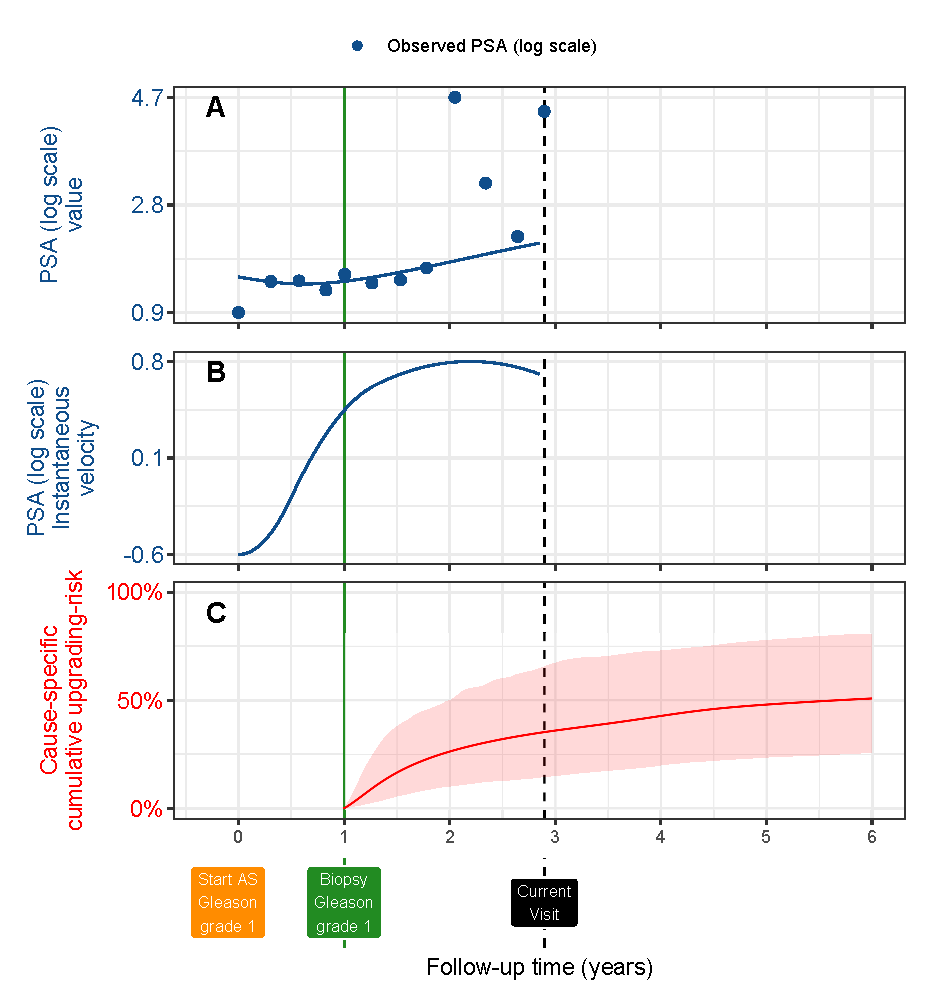
\includegraphics[width=\columnwidth]{images/jmExplanationPlot_113.eps}}
\caption{\textbf{Illustration of the joint model on a real PRIAS patient}. \textbf{Panel~A:} Observed PSA (blue dots) and fitted PSA (solid blue line), log-transformed. \textbf{Panel~B:} Estimated instantaneous velocity of PSA (log-transformed). \textbf{Panel~C}: Predicted cumulative-risk of reclassification (95\% credible interval shaded). Reclassification is defined as an increase in Gleason grade from grade~1 to 2 or higher. This risk of reclassification is available starting from the time of the latest negative biopsy (vertical green line at year 1 of follow-up). The joint model estimated it by combining the fitted value and estimated instantaneous velocity of PSA (log scale), and time of the latest negative biopsy. Black dashed line at year 3 denotes the time of current visit.}
\label{fig:jmExplanationPlot_113}
\end{figure}

\subsection{Risk of Reclassification Based Personalized Biopsies}
The key component in personalized schedules is the cumulative-risk of reclassification. Given, a patient's accumulated PSA measurements and biopsy results, our joint model predicts the cumulative-risk of reclassification at his current as well as future visit times (Panel~C, Figure~\ref{fig:jmExplanationPlot_113}). This cumulative-risk is also updated as more patient data becomes available over follow-up (Figure~5, Supplementary~B).

In PRIAS, patient PSA is measured every 6 months. If during such a visit, a patient's predicted cumulative-risk of reclassification is more than a certain threshold (e.g., 10\%) we schedule an immediate biopsy. Since our model predicted his cumulative-risk at his future follow-up visits as well, we can schedule future biopsies too. We achieve this by repeatedly applying the same risk threshold rule at each future follow-up visit (Supplementary~C). We maintain a minimum gap of one year between consecutive biopsies (PRIAS recommendation). Example personalized schedules based on 5\% and 10\% risk thresholds are shown in Panel~B, Figure~\ref{fig:demo_pat1}.

\begin{figure}[!htb]
\centerline{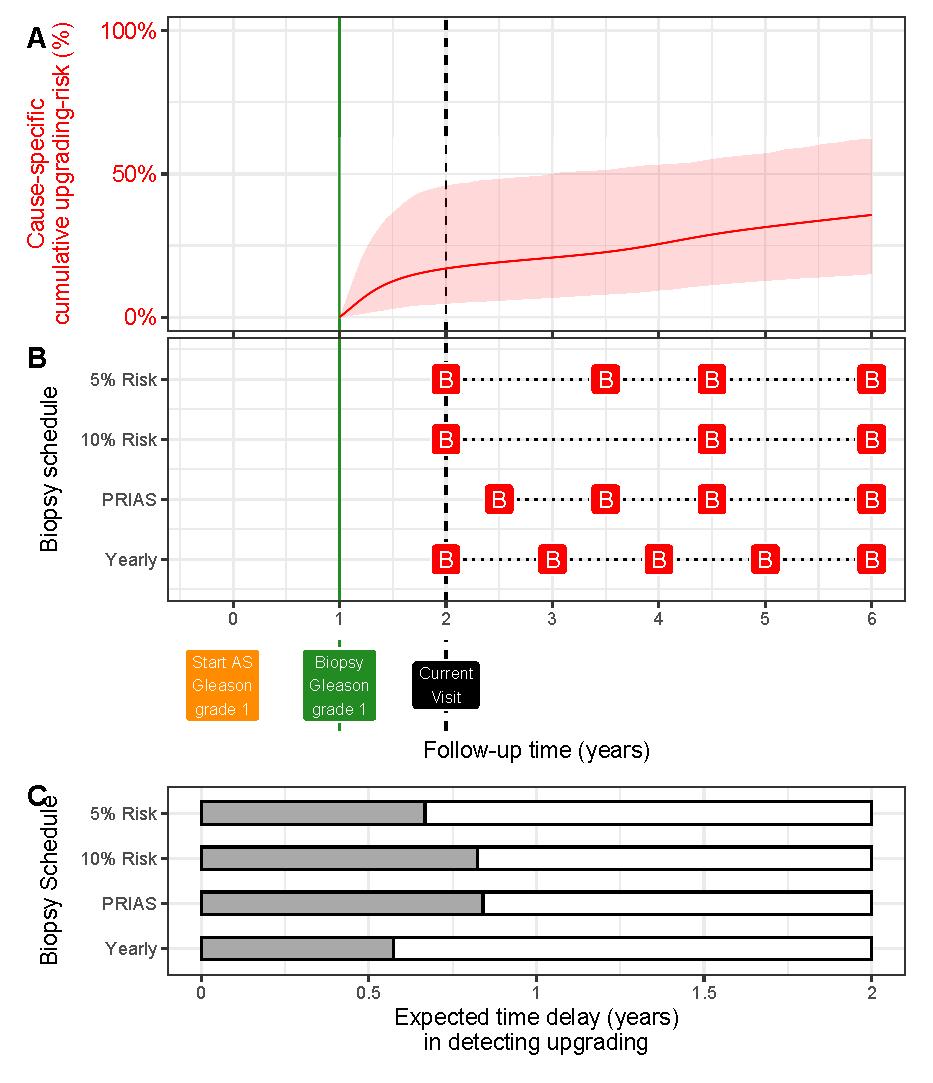
\includegraphics[width=\columnwidth]{images/demo_pat1.eps}}
\caption{\textbf{Illustration of personalized and fixed schedules of biopsies}. The PSA profile of this patient is shown in Figure~\ref{fig:jmExplanationPlot_113}. \textbf{Panel~A:} Predicted cumulative-risk of reclassification (95\% credible interval shaded). \textbf{Panel~B:} Personalized and fixed schedules of biopsies, with a red `B' indicating a scheduled biopsy. \textbf{Panel~C:}\ Expected time delay in detecting reclassification (months) for different schedules. Green vertical line at year 1 denotes the time of latest negative biopsy. Black dashed line at year 3 denotes time of current visit.}
\label{fig:demo_pat1}
\end{figure}

The choice of the risk threshold in the personalized schedule dictates the \textit{consequences} of following that schedule. \textit{Consequences} are, the timing and the total number of biopsies, and the expected delay in detecting reclassification. Our model also estimated these \textit{consequences} in a personalized manner (Panel~B,C in Figure~\ref{fig:demo_pat1}, and Figure~9--11 in Supplementary~C) given any schedule of biopsies. Thus patients can compare fixed schedules with personalized schedules based on different risk thresholds before making a choice.

\subsection{Model Validation}
We validated our model internally as well as externally. Internal validation utilized the PRIAS dataset. External validation was done in largest five AS cohorts of the GAP3 database~\citep{gap3_2018}, namely University of Toronto AS (Toronto), Johns Hopkins AS (Hopkins), Memorial Sloan Kettering Cancer Center AS (MSKCC), King's College London AS (KCL), and Michigan Urological Surgery Improvement Collaborative AS (MUSIC). We assessed our model's ability to discriminate between patients who observe reclassification versus patients who do not observe reclassification, using the area under the receiver operating characteristic curve or AUC~\citep{rizopoulos2017dynamic}. We evaluated the prediction accuracy of our model visually using calibration plots~\citep{royston2013external,steyerberg2010assessing}, and quantitatively via mean absolute prediction error~\citep{rizopoulos2017dynamic}. Due to the longitudinal nature of AS studies, the AUC and prediction error varies over time (Supplementary~B.1). We recalibrated our model's baseline hazard of reclassification in those external cohorts (Supplementary~B.1) where our model was miscalibrated.

\subsection{Web-Application}
We implemented our methodology in a web-application \url{https://emcbiostatistics.shinyapps.io/prias_biopsy_recommender/}. It utilizes our joint model fitted to the PRIAS dataset. Currently, the web-application supports PRIAS and the five external cohorts in which we validated our model. Patient data can be entered manually or can be uploaded in Microsoft Excel format. Predictions for risk of reclassification are shown for a limited follow-up period. This limit varies between cohorts according to their current study period. The web-application allows comparison of the \textit{consequences} of following these schedules: personalized schedules based on 5\%, 10\%, and 15\% risk threshold; annual biopsies; biennial biopsies; and PRIAS schedule.